\documentclass[letterpaper,twocolumn,amsmath,amsfont,amssymb,english,aps,jcp,preprintnumbers,groupaddress,nofootinbib,tightenlines]{revtex4}

\usepackage{graphicx}
\usepackage{epstopdf}

%\documentclass[aps,prb,letterpaper,twocolumn,nofootinbib,showkeys]{revtex4-1}
%\documentclass[aps,amssymb,prl,letterpaper,twocolumn,nofootinbib,showkeys]{revtex4-1}

%\usepackage[backend=bibtex]{biblatex}

%    backend=biber,
%    style=authoryear,
%    natbib=true,
%    sortlocale=en_US,
%    url=false,
%    doi=true,f
%    eprint=false
%]{biblatex}
%\usepackage{hyperref}

\newcommand{\mat}[1]{\boldsymbol{#1}}
\newcommand{\mmat}[1]{\widetilde{\boldsymbol{#1}}}
\newcommand{\matT}[1]{\boldsymbol{#1}^\dagger}
\newcommand{\ot}{ {\scriptstyle \otimes}_{ \tau } }
\newcommand{\ots}{ {\scriptstyle \otimes}_{ \tau_s } }

%\hypersetup{pdftitle={FreeON Project Report 1}}
%\hypersetup{pdfauthor={Matt Challacombe and Nicolas Bock}}
%\hypersetup{pdfsubject={A SpAMM Stabilized Newton Schulz Preconditioner: Fighting Error with Error}}

%\bibstyle{aipnum4-1}

\begin{document}

\title{On Stability of the First Order Newton Schulz Iteration in an Approximate Algebra}

\author{Matt Challacombe}
\email{matt.challacombe@freeon.org}
\homepage{http://www.freeon.org}
\affiliation{Theoretical Division, Los Alamos National Laboratory}

\author{Terry Haut}


\author{Nicolas Bock}
\email{nicolasbock@freeon.org}
\homepage{http://www.freeon.org}
\affiliation{Theoretical Division, Los Alamos National Laboratory}

\begin{abstract}
\end{abstract}

\maketitle
\section{Introduction}

In many areas of application, finite correlations lead to matrices
with decay properties.  By decay, we mean an approximate (perhaps
bounded \cite{}) inverse relationship between matrix elements and an
associated distance; this may be a simple inverse exponential
relationship between elements and the Cartesian distance between
support functions, or it may involve a generalized distance, {\em
  e.g.}~a statistical measure between strings.  In electronic
structure, correlations manifest in decay properties of the gap
shifted matrix sign function, as projector of the effective
Hamiltonian (Fig.~\ref{figure1}).  More broadly, matrix decay
properties may correspond to statistical matrices \cite{penrose1974,
  voit00, Anselin2003, Hardin2013, Krishtal2014}, including learned
correlations in a generalized, non-orthogonal metric \cite{}.  More
broadly still, problems with local, non-orthogonal support are often
solved with congruence transformations of the matrix inverse square
root \cite{Lowdin56, naidu11} or a related factorization
\cite{Krishtal2014}; these transformations correlate local support
with a representation independent form, {\em eg.}~of the eigenproblem.
Interestingly, the matrix sign function and the matrix inverse square
root function are related by Higham's identity:
\begin{equation}
\rm{sign} \left( \begin{bmatrix} 0 & \mat{s}      \\ \mat{I}       & 0\end{bmatrix} \right)  =
                 \begin{bmatrix} 0 & \mat{s}^{1/2} \\ \mat{s}^{-1/2} & 0\end{bmatrix}  .
\end{equation}
A complete overivew of matrix function theory and computation is given
in Higham's enjoyable reference \cite{Higham08}.

A well conditioned matrix $\mat{s}$ may often correspond to matrix
sign and inverse square root functions with rapid exponential decay,
and be amenable to the sparse matrix approximation
$\bar{\mat{s}} = \mat{s}+ \mat{\epsilon}^{\mat{s}}_\tau$,
where $\mat{\epsilon}^{\mat{s}}_\tau$ is the error introduced
according to some criterion $\tau$.  Supporting this approximation are
useful bounds to matrix function elements \cite{Benzi99b, }.
The criterion $\tau$ might be a drop-tolerence,
$\epsilon^{\mat{s}}_{\tau} = \{-s_{ij}*\hat{\mat{e}}_i \, | \, |s_{ij}|<\tau \}$,
a radial cutoff,
$\epsilon^{\mat{s}}_{\tau} = \{-s_{ij}*\hat{\mat{e}}_i \, | \, \lVert \mat{r}_i - \mat{r}_j \rVert > \tau \}$,
or some other approach to truncation, perhaps involving a sparsity
pattern chosen {\em a priori}.
Then, conventional computational kernels may be employed, such as the
sparse general matrix-matrix multiply ($\tt{SpGEMM}$)
\cite{Gustavson78, Toledo97, challacombe00, bowler00}, yielding fast
solutions for multiplication rich iterations and a modulated {\bf
  (what do you mean with modulated?)} fill-in.
These and related incomplete/inexact approaches to the computation of
sparse approximate matrix functions often lead to ${\cal O}(n)$
algorithms, finding wide use in technologically important
preconditioning schemes, the information sciences, electronic
structure and many other disciplines. Comprehensive surveys of these
methods in the numerical linear algebra are given by Benzi
\cite{Benzi99,Benzi02}, and by Bowler \cite{Bowler12} and Benzi \cite{Benzi13}
for electronic structure.

\begin{figure}[t]\label{figure1}
 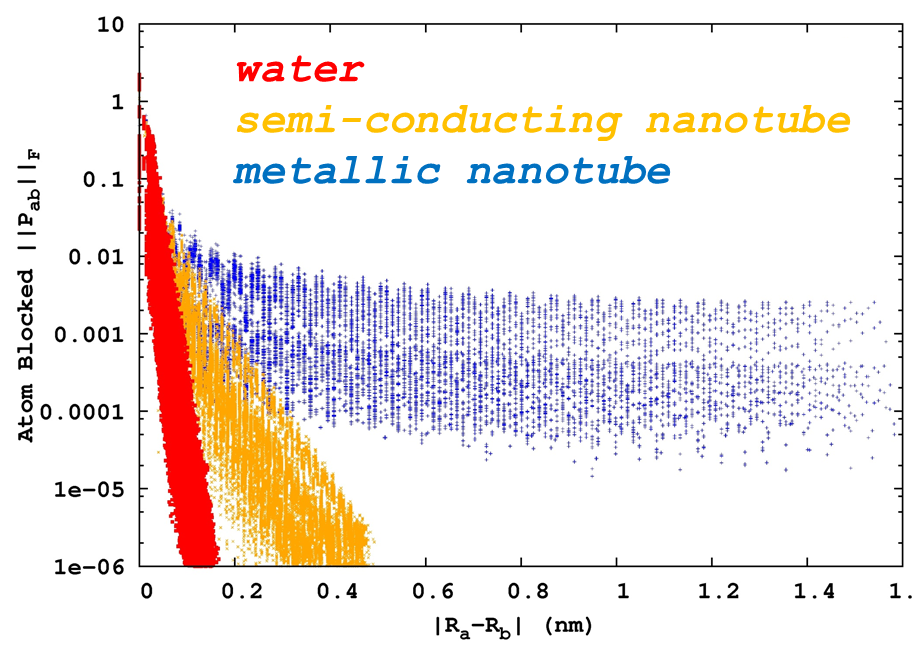
\includegraphics[width=3.5in]{decay_picture.png}
  \caption{Examples from electronic structure of decay for the
    spectral projector (gap shifted sign function) with respect to
    local (atomic) support.  Shown is decay for systems with
    correlations that are short (insulating water), medium
    (semi-conducting 4,3 nanotube), and long (metalic 3,3 nanotube)
    ranged, from exponential (insulating) to algebraic (metallic). }
\end{figure}

Because the truncated multiplication is controlled only by absolute,
additive errors in the product,
\begin{equation} \label{sparseapprox}
\overline{ \mat{a} \cdot \mat{b} }\; = \; \mat{a}\cdot\mat{b} \; +\; \mat{\epsilon}^{\mat{a}}_\tau \cdot \mat{b} \;+\;
 \mat{a} \cdot \mat{\epsilon}^{\mat{b}}_\tau  \; + \;   {\mathcal O}(\tau^2)
\end{equation}
achieving sparse, stable and rapidly convergent iteration for
ill-conditioned problems can be challenging \cite{}.  In cases of
extreme degeneracy, hierarchical semi-seperable (reduced rank)
algorithms can offer effective complexity reduction \cite{}.  However,
many practical cases are somewhere in-between sparse and meaningfully
degenerate regimes; effectively dense but without an exploitable
reduction in rank.  This is the case in electronic structure for
strong but non-metallic correlation, {\em e.g.}~towards the Mott
transition \cite{}, and also in the case of local atomic support
towards completeness \cite{Others, Hutter, Gigi}.

\pagebreak

\section{Sparse Approximate Matrix Multiplication}

In this contribution, we consider an $N$-body approach to the
approximation of matrix functions with decay, based on the quadtree
data structure \cite{wise, samet}
\begin{equation}
\mat{a}^i = \begin{bmatrix} \,  \mat{a}^{i+1}_{00} \, & \,  \mat{a}^{i+1}_{01} \,  \\[0.2cm]  \, \mat{a}^{i+1}_{10} \,  & \,\mat{a}^{i+1}_{11} \, \end{bmatrix} \, ,
\end{equation}
{\bf (I know we argued about this before, but I still like the normal 1-based notation better :) )}
and orderings that are locality preserving \cite{}.  Orderings that
preserve data locality are well developed in the database theory
\cite{}, providing fast spatial and metric queries.  Locality
enabled, fast data access is central to the $N$-Body approximation
\cite{}, and an important problem for enterprise \cite{} and runtime
systems \cite{}, with memory hierarchies becoming increasingly
asynchronous and decentralized \cite{cache}.  For matrices with
decay, orderings that preserve locality lead to blocked-by-magnitude
matrix structures with well segregated neighborhoods, inhabited by
matrix elements of like size, and efficiently resolved by the quadtree
data structure \cite{}.

\subsection{Stable $\tt SpAMM$}

With blocked-by-magnitude ordering of matrices $\mat{a}$ and
$\mat{b}$, the Sparse Approximate Matrix Multiplication ($\tt SpAMM$)
kernel, $\ot$, carries out fast occlusion culling of insignificant
volumes in the product octree:
\begin{widetext}
\begin{equation}
\mat{a}^{i} \ot \mat{b}^{i} =
\left\{
        \begin{array}{ll}
                 \emptyset \quad \tt{if}\quad \lVert \mat{a}^i \rVert \lVert \mat{b}^i \rVert < \tau \lVert a \rVert \lVert b \rVert \\[0.2cm]
                 \mat{a} ^i \cdot \mat{b}^i \quad  \tt{if}(i=\tt{leaf}) \\[0.2cm]
\begin{bmatrix} \mat{a}^{i+1}_{00} \ot \mat{b}^{i+1}_{00} +\mat{a}^{i+1}_{01} \ot \mat{b}^{i+1}_{10} \; , \; &
                \mat{a}^{i+1}_{00} \ot \mat{b}^{i+1}_{01} +\mat{a}^{i+1}_{01} \ot \mat{b}^{i+1}_{11}  \\[0.2cm]
                \mat{a}^{i+1}_{00} \ot \mat{b}^{i+1}_{01} +\mat{a}^{i+1}_{01} \ot \mat{b}^{i+1}_{11} \; , \; &
                \mat{a}^{i+1}_{00} \ot \mat{b}^{i+1}_{01} +\mat{a}^{i+1}_{01} \ot \mat{b}^{i+1}_{11}
\end{bmatrix}  \quad \tt{else}
                \end{array}
              \right.  \, ,
\end{equation}
\end{widetext}
with errors linear in $\tau$ bounded by the sub-multiplicative norms
$\lVert \cdot \rVert \equiv \lVert \cdot \rVert_F$ and the
Cauchy-Schwarz inequality \cite{kahan,}.

The approximate $\tt SpAMM$ product is
\begin{equation}
\widetilde{\mat{a}\cdot \mat{b}} \,  \equiv \, \mat{a} \ot \mat{b} \,
  = \, \mat{a} \cdot \mat{b} + \mat{\Delta}^{a \cdot b}_{\tau}
%+ {\cal{O}} \left(  \tau^2 \right) \; ,
\end{equation}
with the culled contractions $\mat{\Delta}^{a \cdot b}_{\tau}$ obeying
the $\tt SpAMM$ bound
\begin{equation}\label{bound}
\lVert \mat{\Delta}^{a \cdot b}_{\tau} \rVert \, \leq \, \tau \, \lVert \mat{a} \rVert  \,  \lVert \mat{b} \rVert \, ,
\end{equation}
at each level of recursion.  This makes $\ot$ {\em stable}, as defined
by Demmel, Dumitriu and Holz (DDH; Ref.~\cite{Demmel07}).  However,
instead of the roundoff error, we are concerned with a deterministic
$\tt SpAMM$ error%
\footnote{A non-deterministic ${\tt SpAMM}$ occlusion error is also
  possible, {\em e.g.} associated with probabilistic stabilization
  \cite{} or sampling \cite{} methods.},
which leads to a non-associative algebra and error flows with
properties of the Lie bracket
\begin{equation} \label{braket}
\widetilde{\left[ \mat{a} , \mat{b} \right]} \equiv \mat{a} \ot \mat{b}-\mat{b} \ot \mat{a}
=  \left[ \mat{a} , \mat{b} \right]
+ \mat{\Delta}^{a\cdot b}_{\tau} -\mat{\Delta}^{b\cdot a}_{\tau} \,.
\end{equation}

%%<<<<<<< HEAD
\subsection{Related Research} 

Here, we note overlaping themes and research related to the results presented here.
First,  its worth noting that the $\tt SpAMM$ concept has evolved, 
from a row-coloum based occlusion \cite{}, to recursive octree occlusion \cite{}, and in this work, to the
bounded (stable) occlusion satisfying Eq.~\ref{bound}.    This evolution cooresponds to an  ongoing economization and radical simplification
of strongly interacting,  high performance solvers in the $\tt freeon$ ecosystem \cite{}.  These economizations 
include $n$-body algorithms for the five common electronic structure solvers \cite{}, 
and the (ongoing) development of generic strategies supporting rapid, hierarhcical access of spatial and metric data \cite{sammet, wise}.  
For example, $\tt SpAMM$ has been extended to the {\em triple} metric querry for hextree occlusion of 
the exact Fock exchange \cite{}.  

$\tt SpAMM$ is broadly related to {\em generalized n-body} methods, poularized by Grey \cite{},  
that are simply algorithms based on fast (hierarchical) spatial and metric querry \cite{Sammet} together with local approximation \cite{}.  
Recently, x, y  and Yellik showed perfect strong scaling and communication optimality 
for pairwise $n$-body methods \cite{Warren Salmon, Yellik}.  Also Demmel and showed  for the related fast matrix multiplicaiton.
It may be possible to show similar results, based on the locality of reference developed in this work, encompassing both 
strong Euclidian locality and with algebraic (diagonal) locality towards identity.  

As noted by Aluru \cite{}, the top-down $n$-body model and breadth-first map-reduction are equivalent \cite{}, offering
the potential for alignment with emergent enterprise frameworks \cite{} and functional programming 
languages that support generacity \cite{}. Language support for generic recursion may allow very complex solver ecosystems 
with very simple (skeletonized) frameworks, lowering barriers to entry, enhancing performance towards decentralized memory landscapes, 
and following a sustainable commodity trend \cite{softwaresustainanbilty} that offers 
increasingly cheap compute cycles over the next few decades \cite{}. 

$\tt SpAMM$ is perhaps most closely related to the Strassen-like branch of fast matrix multiplication \cite{},  
which has been on fire with recent new developments \cite{}.  In the Strassen-like approach, disjoint volumes in (abstract) tensor 
intermediates are omitted recursively \cite{}.  In the $\tt SpAMM$ approach to fast multixplication, a volume of
significant contributions is culled from the naive $ijk$-cube of the intermediate contraction, 
with error bounded by Eq.~\ref{bound}.  These approaches would seem to be compatible and synergystic.

$\tt SpAMM$ is also related to technologies for the non-deterministic,  compresive sampling of the product.  These 
technologies have also seen exciting developments, including  sketching \cite{Kutzkov2012, Pagh2013}, joining, sensing and probing \cite{}.
These methods involve a wheighted (probablistic) and on the fly sampling with the potential for complexity reduction under
certain assumptions (random distributions) [{\bf is this true for all? what about MAD?}].  
$\tt SpAMM$ also employs an on the fly wheighted sampling, based on the product of matrix norms, 
but opperating under the contrary assumption of compresion through locality in the naive $ijk$ space, brought about 
via correlations in the algebra (towards identity) and in the underlying data (blocked-by-magnitude).

Methods that achieve compression in the product stream are different from reduced rank algorithms that achieve 
matrix compression \cite{} and/or sparsificiation \cite{} of the matrix in a step preceeding multiplication.  
However, these approaches are not incompatible, with the quadtree data structure supportive 
of most approaches to matrix compression \cite{} and sparsification \cite{wise}, as well as most 
fast solvers they might interact with.  With little deflation in the cost of fast memory, solver ecosystems 
that can bring multiple levels of approximation to in place data may enjoy significant cumulitive advantages. 

Finally, the mathematical developments in Higham, Mackey, Mackey and T (HMMT; Ref.~\cite{}) demonstrate 
the convergence of NS iteration under all groups, addressing potential failure due to the development of 
pathalogical symmetries related to {\em e.g.} Eq.~\ref{braket}.    Also in this key paper, HMMT develop
the fixed point stability analyses (about 2/3 of the way in), which this work draws heavily upon.  This 
work also draws on the scaling in Chen and Chow's \cite{} approach to a scaled NS iteration for ill-conditioned 
problems. 

% like the Hiearchical Semi-Seperable method, 
% but are similar in structure, complimentary and synergistic. 

% In this work, we are focused on achieving preconditioned (lensed) states for $\ot$ at the edge of stability,  
% with future work examining sandwich techniques for achieving additional (full) precision \cite{}.  
% =======
% \subsection{Related Research}

% Here, we note overlaping themes and research related to the results
% presented here.  First, its worth noting that the $\tt SpAMM$ concept
% has evolved, from a row-column based occlusion \cite{}, to recursive
% octree occlusion \cite{}, and in this work, to the bounded (stable)
% occlusion satisfying Eq.~\ref{bound}.  This evolution corresponds to
% an ongoing economization and radical simplification of strongly
% interacting, high performance solvers in the $\tt FreeON$ ecosystem
% \cite{}.  These economizations include $N$-body algorithms for the
% five common electronic structure solvers \cite{}, and the (ongoing)
% development of generic strategies supporting rapid, hierarchical
% access of spatial and metric data \cite{sammet, wise}.  For example,
% $\tt SpAMM$ has been extended to the {\em triple} metric query for
% hextree occlusion of the exact Fock exchange \cite{}.

% $\tt SpAMM$ is broadly related to {\em generalized N-body} methods,
% popularized by Grey \cite{Gray2001,Gray2003}, that are simply algorithms based on fast
% spatial and metric query \cite{Sammet} together with local approximation
% \cite{}.  Recently, x, y and Yellik derived perfect strong scaling
% communication optimal bounds for pairwise $N$-body methods
% \cite{10.1109/IPDPSW.2012.303}.  Also, Demmel \emph{et al.}~derived such
% bounds for the related fast matrix multiplication.  
% \cite{Solomonik2011}

% It may be possible
% to show similar results for $\tt SpAMM$, by exploiting the additional
% locality of reference developed in this work, {\em e.g.}~based on
% strong Euclidean locality and with iteration towards the identity.

% As noted by Aluru \cite{}, the top-down $N$-body model and
% breadth-first map-reduction are equivalent \cite{}, offering the
% potential for alignment with emergent enterprise frameworks \cite{}
% and functional programming languages that support generacity
% \cite{}. Language support for generic recursion may allow very complex
% solver ecosystems with very simple (skeletonized) frameworks, lowering
% barriers to entry, enhancing performance towards decentralized memory
% landscapes, and following a sustainable commodity trend
% \cite{softwaresustainanbilty} that offers increasingly cheap compute
% cycles over the next few decades \cite{}.

% $\tt SpAMM$ is perhaps most closely related to the Strassen-like
% branch of fast matrix multiplication
% \cite{springerlink:10.1007/BF02165411}, which has been on fire with
% recent new developments \cite{Ballard2014}.  In the Strassen-like
% approach, disjoint volumes in (abstract) tensor intermediates are
% omitted recursively \cite{}.  In the $\tt SpAMM$ approach to fast
% multixplication, a volume of significant contributions is culled from
% the naive $ijk$-cube of the intermediate contraction, with error
% bounded by Eq.~\ref{bound}.  These approaches would seem to be
% compatible and synergistic.

% $\tt SpAMM$ is also related to database problems involving the 
% join \cite{Mishra92,Hoel94,Jacox03,Chen07,Amossen09,Lieberman08,Kim09}, and also 
% the matrix sketch  \cite{Sarlos2006,Drineas2006,Mahoney2012,Pagh2013,Sivertsen2014,Woodruff2015}.
% These methods deliver a relative, probabilistic error 
% and on the fly sampling with the potential for complexity reduction under {\em randomization}.
% $\tt SpAMM$ delivers a rigorous relative error bound and on the fly weighted sampling, 
% but operates under the contrary assumption of compression through {\em correlations}
% in the naive $ijk$ space, brought about via lensing (algebraic localization cooresponding to identity iteration),
% and for matrices with decay, by strong metric (block-by-magnitude) locality in the underlying data. 

% Methods that achieve compression in the product stream are different
% from reduced rank algorithms that achieve compression \cite{}
% and/or sparsificiation \cite{} of the matrix in a step preceding
% multiplication.  However, these approaches are not incompatible, with
% the quadtree data structure supportive of most approaches to matrix
% compression \cite{} and sparsification \cite{wise}, as well as most
% fast solvers they might interact with.  With little deflation in the
% cost of fast memory, solver ecosystems that can bring multiple levels
% of approximation to in-place data may enjoy significant cumulative
% advantages.

% Finally, the mathematical developments in Higham, Mackey, Mackey and
% Tisseur (HMMT; Ref.~\cite{Higham2005}) demonstrate the convergence of
% Newton-Schulz (NS) iteration under all groups, addressing potential
% failure due to the development of pathalogical symmetries related to
% {\em e.g.}~Eq.~\ref{braket}.  Also in this key paper, HMMT develop the
% fixed point stability analysis (about 2/3 of the way in), which this
% work draws heavily upon.  This work also draws on the scaling in Chen
% and Chow's \cite{} approach to a scaled NS iteration for
% ill-conditioned problems.

% % like the Hiearchical Semi-Seperable method,
% % but are similar in structure, complimentary and synergistic.

% % In this work, we are focused on achieving preconditioned (lensed) states for $\ot$ at the edge of stability,
% % with future work examining sandwich techniques for achieving additional (full) precision \cite{}.



% >>>>>>> d4c0ab84d18629f0a3f1847549c555b7d8eece61

% Targeted at the preconditioned state: diff factorization and solution of the inverse via SPAI. This
% approach has the lower dependence on the $\kappa(\mat{s})^{-1/2}$ instead of $\kappa(\mat{s})^{-1}$
% cost of factorization  Because computing residual corrected .

% $\tt SpAMM$ is {\em not} an on the fly matrix truncation/sparsification algorithm \cite{}, and shouldn't be associated


% with algorithms based on the blocked-CSR (BCSR) and distributed-blocked-CSR (DBCSR) structures,
% introduced previously by one of us \cite{}.


%In the case of $\tt SpAMM$,  querries are performed on the norm (matrix distance),
%rather than a Euclidean distance, as in the case of {\em e.g.}~an astrophisical tree code \cite{}.
%Also, our recursive approximation is occlusion via the Cauchy-Schwarz
%inequality and the sub-multiplicative property, rather than local Taylor expansion.

\section{First Order Newton-Shulz Iteration}

There are two common, first order NS iterations; the sign iteration
and the square root iteration, related by the square, $\mat{I}\left(
\cdot \right)= {\rm sign}^2\left( \cdot \right) $.  These equivalent
iterations converge linearly at first, then enter a basin of stability
marked by super-linear convergence.  Our interest is to access this
basin with the most permissive $\tau$ possible, building a foundation
for future refinement
%, {\em e.g.}
at a reduced cost and with a higher precision ($\tau \rightarrow 0$)
\cite{MChallacombe16}.

\subsection{Sign iteration}

For the NS sign iteration, this basin is marked by a behavioral change
in the difference $\delta \mat{X}_k = \widetilde{\mat{X}}_k -\mat{X}_k
= {\rm sign} \left(\mat{X}_{k-1}+\delta \mat{X}_{k-1} \right) -{\rm
  sign} \left(\mat{X}_{k-1} \right)$, where $\delta \mat{X}_{k-1}$ is
some previous error.  The change in behavior is associated with the
onset of idempotence and the bounded eigenvalues of ${\rm sign}'\left(
\cdot \right)$, leading to stable iteration when ${\rm sign}'\left(
\mat{X}_{k-1} \right) \delta \mat{X}_{k-1} < 1 $.  Global perturbative
bounds on this iteration have been derived by Bai and Demmel
\cite{Bai98usingthe}, while Byers, He and Mehrmann \cite{} developed
asymptotic bounds.  The automatic stability of sign iteration is a
well developed theme in Ref.\cite{Higham08}.

\subsection{Square root iteration}

In this work, we are concerned with resolution of the identity \cite{}
\begin{equation}
\mat{I} \left( \mat{s} \right) =\mat{s}^{1/2} \cdot \mat{s}^{-1/2} \, ,
\end{equation}
and the cooresponding canonical (dual) square root iteration \cite{};
\begin{eqnarray}\label{cannonical}
\mat{y}_k &\leftarrow& h_\alpha \left[ \mat{y}_{k-1} \cdot \mat{z}_{k-1} \right] \cdot \mat{y}_{k-1}  \nonumber \\
\mat{z}_k &\leftarrow& \mat{z}_{k-1} \cdot h_\alpha \left[ \mat{y}_{k-1} \cdot \mat{z}_{k-1} \right] \; ,
\end{eqnarray}
with eigenvalues in the proper domain aggregated towards 0 or 1 by the
NS map $h_\alpha[\mat{x}]=\frac{\sqrt{\alpha}}{2} \left(3-\alpha
\mat{x} \right)$ \cite{}.  Then, starting with $\mat{z}_0=\mat{I}$ and
$\mat{x}_0=\mat{y}_0=\mat{s}$, ${\mat{y}}_k \rightarrow
\mat{s}^{1/2}$, ${\mat{z}}_k \rightarrow \mat{s}^{-1/2}$ and
${\mat{x}}_k \rightarrow {\mat{I}}$.  As in the case of sign
iteration, this dual iteration was shown by Higham, Mackey, Mackey and
Tisseur \cite{Higham2005} to remain bounded in the superlinear regime,
by idempotent Frechet derivatives about the fixed point
$\left(\mat{s}^{1/2},\mat{s}^{-1/2}\right)$, in the direction $\left(
\delta \mat{y}_{k-1} , \delta \mat{z}_{k-1} \right)$:
\begin{eqnarray}
\delta \mat{y}_k &=& \frac{1}{2} \delta \mat{y}_{k-1} - \frac{1}{2} \mat{s}^{1/2} \cdot \delta \mat{z}_{k-1} \cdot \mat{s}^{1/2} \\
\delta \mat{z}_k &=& \frac{1}{2} \delta \mat{z}_{k-1} - \frac{1}{2} \mat{s}^{-1/2} \cdot \delta \mat{y}_{k-1} \cdot \mat{s}^{-1/2} \;.
\end{eqnarray}
In this contribution, we consider another aspect of convergence,
namely the (hopefully) linear approach towards stability of the
iteration
\begin{equation}
\widetilde{\mat{x}}_k \leftarrow
 \widetilde{\mat{y}}_k \left( \widetilde{\mat{x}}_{k-1} \right)
\, \ot \, \widetilde{\mat{z}}_k \left( \widetilde{\mat{x}}_{k-1} \right) \, ,
\end{equation}
made difficult by ill-conditioning and a sketchy $\ot$.

\subsection{the NS map}

Initially, $h'_\alpha$ at the smallest eigenvalue $x_0$ controls the
rate of progress towards idempotence.  As recently shown by Jie and
Chen \cite{Chen2014}, for very ill-conditioned problems, a factor of
two reduction in the number of NS steps can be achieved by choosing
$\alpha \sim 2.85$, which is at the edge of stability.  As argued by
Pan and Schreiber \cite{Pan1991}, Jie and Chen \cite{Chen2014},
switching or damping the scaling factor towards $\alpha=1$ at
convergence is important, shifting emphasis away from the behavior of
$x_0$ towards {\em e.g.}~$x_i \in [0.01,1]$, emphasizing overall
convergence of the broad distribution \cite{Pan and Scriber}.  In an
approximate algebra like $\tt SpAMM$, the potential for eigenvalues to
fluctuate out of the domain of convergence must be considered.  This
is addressed in Section \ref{}.

\subsection{Ill-conditioning, Stability and Implementation}

There are a number of nominally equivalent instances of the square root iteration, related by commutations and transpositions. 
However, these instances may have very different stability properties,  controled to first order by the Frechet derivatives
\begin{equation}
  \mat{x}_{\delta \widehat{ \mat{y}}_{k-1}}
= \lim_{\tau \rightarrow 0} \slantfrac{ \mat{x} \left( \mat{y}_{k-1} + \tau \delta \widehat{\mat{y}}_{k-1} ,  {\mat{z}}_{k-1}  \right)
                                     -\mat{x}_k    }{\tau} 
 \end{equation}
and
 \begin{equation}
 \mat{x}_{\delta \widehat{ \mat{z}}_{k-1}} = \lim_{\tau \rightarrow 0}
\slantfrac{ \mat{x} \left( {\mat{y}}_{k-1} , \mat{z}_{k-1} +\tau  \delta \widehat{\mat{z}}_{k-1} \right) - \mat{x}_k   }{\tau}  \, , 
 \end{equation}
along the unit directions of the previous errors $\delta \widehat{\mat{y}}_{k-1}$ and $\delta \widehat{\mat{z}}_{k-1}$, corresponding 
to the associated displacement magnitudes $\delta y_{k-1} = \lVert \delta \mat{y}_{k-1} \rVert$  and  $\delta z_{k-1}=\lVert \delta \mat{z}_{k-1} \rVert$.
Then, the differential 
\begin{equation} \label{firstorderdual}
\delta \mat{x}_k = \,  { \mat{x}}_{\delta \widehat{\mat{y}}_{k-1}}  \, {\scriptstyle \times} \, \delta y_{k-1}
                 \, + \,  { \mat{x}}_{\delta \widehat{\mat{z}}_{k-1}}  \, {\scriptstyle \times} \, \delta z_{k-1}  \, + {\cal O}(\tau^2) 
\end{equation}
determines the total first order stability. 

This formulation allows to consider orientational effects involving eigenvector fidelity and convergence of 
derivatives towards zero seperately from displacement effects involving accumulation and $\tt SpAMM$ source errors.
In some cases, instabilities may be associated with derivatives that do not vanish towards identity, yeilding an unbounded iteration \cite{}.
In other instances, an instability may be associated with rapidly increasing displacements, due to a too large $\tau$.  Instability 
may also arize due to the numerical corruption of the eigenvectors, also resulting in derivatives that vanish too slowly (or blow up altogether).    

The potential for
instability is increased with ill-conditioning through the terms $\lVert \mat{z}_{k} \rVert  \rightarrow \sqrt{\kappa\left(\mat{s} \right)}$.
Also for ill-conditioned systems, scaling is nessesary to accelerate convergence.  However with scaling, increasing the map 
derivative $h'_\alpha$ can also further enhance the rate of error accumulation. 

In following sections, we'll examine how these effects differ from the ideal (double precision) cannonical (dual) square root iteration
for ill-conditioned systems and in the strongly non-associative, sketchy $\ot$ regime corresponding to permisive values of $\tau$.
At this early stage, we are interested in hazzards and opportunities associated with
different formulations and implementational details.   In addition to deviations from the full precision dual instance,
we will develop the  ``stabilized'' instance,
\begin{eqnarray}\label{stabilized}
\mat{z}_k &\leftarrow& \mat{z}_{k-1} \cdot h_\alpha \left[ \mat{x}_{k-1} \right] \; , \nonumber \\
\mat{x}_k &\leftarrow&  \mat{z}^\dagger_{k} \cdot \mat{s} \cdot \mat{z}_{k-1} \; ,
\end{eqnarray}
with the corresponding differential;
\begin{equation} \label{firstorderstab}
\delta \mat{x}_k = \,  { \mat{x}}_{\delta \widehat{\mat{z}}_{k-1}}  \, {\scriptstyle \times} \, \delta z_{k-1}  \, + {\cal O}(\tau^2)  \, .
\end{equation}


Nominally, $\mat{y}^{\rm dual}$ is equivalent to $\mat{y}^{\rm stab}_k \equiv \mat{z}^\dagger_{k} \cdot \mat{s}$ 
is also equivalent to $\mat{y}^{\rm naive}_k \equiv \mat{z}_{k} \cdot \mat{s}$.
However, with ill-conditioning and in only double precision, these two instances may diverge due to non-associative errors that rapidly compound.
In the case of the duals iteration under $\tt SpAMM$ approximation, the $\widetilde{\mat{y}}^{\rm dual}_k$ channel does not retain contact 
with the eigenvectors, span $\mat{s}$, whilst the stab instance does.  
In the duals iteration, the $\widetilde{\mat{y}}_k$  $\tt SpAMM$ update 
is mild, with errors in the relative product remaining well conditioned.  
In the stab instance, conection with $\mat{s}$ is retained at each step, but at the price of the 
$\mat{y}^{\rm stab}_k$ update involving magnitudes that vary widely in the $\tt SpAMM$ product.     

For these reasons, maintaining connection to the eigenvectors of $\mat{s}$ through 
a tighter first product is nessesary.  In the stab instance, and with a 
tighter ``{\em s}'' product, $\tau_s \ll \tau$, we find very interesting left/right differences; 
namely, the right first product 
\begin{equation} 
\widetilde{\mat{x}}^R_k \leftarrow \widetilde{\mat{z}}^\dagger_{k} \, \ot  \, \left( \mat{s} \,  \ots \, \widetilde{\mat{z}}_{k-1}  \right) \; ,
\end{equation}
is  different from the left first product 
\begin{equation} 
\widetilde{\mat{x}}^L_k \leftarrow \left(  \widetilde{\mat{z}}^\dagger_{k} \, \ots \, \mat{s} \right) \,  \ot  \, \widetilde{\mat{z}}_{k-1} \; .
\end{equation}

\section{Implementation}

\subsection{programming}

FP, F08, OpenMP 4.0
In the current implementation, all persistence data
(norms, flops, branches \& {\em etc.}) are accumulated compactly in the backward recurrence.  This persistence data
 that may be achieved by minimal locally essential trees \cite{}.


\subsection{scaling and stabilization}

\subsection{regularization}
damping the inversion and the small value to be added c is called Marquardt-Levenberg coefficient

\subsection{convergence}

Map switching and etc based on TrX

\section{Data}

\subsubsection{double exponential ill-conditioning}
3,3 carbon nanotube with diffuse $sp$-function
double exponential (Fig.)

\subsubsection{three-dimensional, periodic}
%\subsubsection{water boxes}
%\subsubsection{ordering}
\subsubsection{Matrix Market}


\section{Results}

\subsection{Stability (Proof)}


\subsection{Error Flows in Square Root Iteration}

\subsubsection{The cannonical (dual) instance}
 
Refering back to Eq.~( \ref{firstorderdual} ), we develop the Fr\'{e}chet analyses \cite{} with the goal of understanding
the contractive approach to identity in competition with error accumulations and $\tt SpAMM$ sources.
Of interest are the derivatives 

% \begin{equation}
%   \mat{x}_{\delta \widehat{ \mat{y}}_{k-1}}
% =   \mat{y}_{\delta \widehat{ \mat{y}}_{k-1}} \cdot \mat{z}_{k}  + \mat{y}_{k}  \cdot \mat{z}_{\delta \widehat{ \mat{y}}_{k-1}}
%  \end{equation}
% and
%  \begin{equation}
%  \mat{x}_{\delta \widehat{ \mat{z}}_{k-1}} =
% \mat{y}_{\delta \widehat{ \mat{z}}_{k-1}} \cdot \mat{z}_{k}  + \mat{y}_{k}  \cdot \mat{z}_{\delta \widehat{ \mat{z}}_{k-1}} \, .
%  \end{equation}


% For $\mat{x}_{\delta \widehat{ \mat{y}}_{k-1}}$ we have
% \begin{multline}
%  \mat{y}_{\delta \widehat{ \mat{y}}_{k-1}} = h_\alpha \left[ \mat{x}_{k-1} \right] \cdot \delta \widehat{\mat{y}}_{k-1} \\
%                                      + h'_\alpha \cdot \delta \widehat{\mat{y}}_{k-1} \cdot \mat{z}_{k-1} \cdot \mat{y}_{k-1}
% \end{multline}
% and
% \begin{equation}
%  \mat{z}_{\delta \widehat{ \mat{y}}_{k-1}} =  \mat{z}_{k-1} \cdot h'_\alpha \delta \widehat{\mat{y}}_{k-1} \cdot \mat{z}_{k-1}
% \end{equation}
% yeilding
% Also, for $\mat{x}_{\delta \widehat{ \mat{z}}_{k-1}}$ we have
% \begin{equation}
%  \mat{y}_{\delta \widehat{ \mat{z}}_{k-1}} =  {\mat{y}}_{k-1} \cdot  h'_\alpha \delta \widehat{ \mat{z}}_{k-1} \cdot  \mat{y}_{k-1}
% \end{equation}
% and
% \begin{multline}
%  \mat{z}_{\delta \widehat{ \mat{z}}_{k-1}} = \delta \widehat{\mat{z}}_{k-1} \cdot   h_\alpha \left[ \mat{x}_{k-1} \right] \\
%                                      + \mat{z}_{k-1} \cdot {\mat{y}}_{k-1} \cdot h'_\alpha \delta \widehat{\mat{z}}_{k-1}  \; ,
% \end{multline}
% yeilding


\begin{multline}
  \mat{x}_{\delta \widehat{ \mat{y}}_{k-1}} = h_\alpha \left[ \mat{x}_{k-1} \right]  \cdot \delta \widehat{\mat{y}}_{k-1} \cdot \mat{z}_{k} \\
 +  h'_\alpha  \delta \widehat{\mat{y}}_{k-1} \cdot \mat{z}_{k-1} \cdot  \mat{y}_{k-1} \cdot  \mat{z}_{k} \\
 + \mat{y}_{k} \cdot \mat{z}_{k-1} \cdot h'_\alpha \delta \widehat{\mat{y}}_{k-1} \cdot \mat{z}_{k-1}  \, .
\end{multline}


\begin{multline}
 \mat{x}_{\delta \widehat{ \mat{z}}_{k-1}} =  {\mat{y}}_{k-1} \cdot  h'_\alpha \delta \widehat{ \mat{z}}_{k-1} \cdot  \mat{y}_{k-1}  \cdot \mat{z}_{k} \\
\qquad + \mat{y}_k \cdot  \delta \widehat{\mat{z}}_{k-1} \cdot   h_\alpha \left[ \mat{x}_{k-1} \right] \\
\qquad \qquad +  \mat{y}_{k} \cdot  \mat{z}_{k-1} \cdot {\mat{y}}_{k-1} \cdot h'_\alpha \delta \widehat{\mat{z}}_{k-1} \, .
\end{multline}

Closer to a fixed point orbit,  $\mat{y}_k \cdot \mat{z}_{k-1} \rightarrow \mat{I}$, $\mat{y}_{k-1} \cdot \mat{z}_{k} \rightarrow \mat{I}$,
$h_\alpha \left[ \mat{x}_{k} \right] \rightarrow \mat{I}$ and $h'_\alpha \rightarrow - \frac{1}{2}$ \cite{higham2005}.  Then,

\begin{equation} \label{yorbit}
 \mat{x}_{\delta \widehat{ \mat{y}}_{k-1}} \rightarrow \delta \widehat{\mat{y}}_{k-1} \cdot \left( \mat{z}_k-\mat{z}_{k-1} \right)
\end{equation}
and
\begin{equation} \label{zorbit}
 \mat{x}_{\delta \widehat{ \mat{z}}_{k-1}} \rightarrow \left( \mat{y}_k-\mat{y}_{k-1} \right) \cdot \delta \widehat{\mat{z}}_{k-1} .
\end{equation}
Thus, contributions along $\delta \widehat{\mat{y}}_{k-1}$ and $\delta \widehat{\mat{z}}_{k-1}$ are tightly shut down in the 
region of superlinear convergence.  Achieving a contractive fixed point orbit, however requires that the three terms in Eq.~(\ref{}),  
with potentially different error accumulations and $\tt SpAMM$ sources, must cancel faster than $\delta y_{k-1}$ 
and $\delta z_{k-1}$ accumulate.

In this analysis, we've seperated the directional component of the error from its distance, because in addition to the
previous compounding error, each displacement contains also a first order $\tt SpAMM$ source error.  Its simpler to 
consider these effects serpately, at least in this first contribution. 

To understand $\delta \mat{z}_{k-1}$, we partially unwind the approxinate  $\widetilde{\mat{z}}_{k-1}$;
%\begin{equation}
\begin{eqnarray} \label{widetildez}
 \widetilde{\mat{z}}_{k-1} &=&  \widetilde{\mat{z}}_{k-2}  \, \ot \, h_\alpha[\widetilde{\mat{x}}_{k-2}]\\
&=& \Delta^{\widetilde{\mat{z}}_{k-2} \cdot h_\alpha \left[ \widetilde{\mat{x}}_{k-2}\right]}_\tau
+ \widetilde{\mat{z}}_{k-2} \cdot h_\alpha\left[ \widetilde{\mat{x}}_{k-2}\right]
%\end{equation}
\end{eqnarray}
Then, using
\begin{equation}
  h_\alpha \left[ \widetilde{\mat{x}}_{k-2} \right]
=  h_\alpha \left[ \mat{x}_{k-2} \right] +  h'_\alpha  \delta \mat{x}_{k-2} \, 
\end{equation}
and taking $\mat{z}_{k-1}$ from both sides, we find  
%Eq.~(\ref{widetildez}) yeilds 
\begin{multline}
 \delta {\mat{z}}_{k-1} =\Delta^{\widetilde{\mat{z}}_{k-2} \cdot h_\alpha \left[ \widetilde{\mat{x}}_{k-2}\right]}_\tau
\\ +\delta \mat{z}_{k-2} \cdot h_\alpha \left[\widetilde{\mat{x}}_{k-2} \right]
+ \mat{z}_{k-2} \cdot h'_\alpha \delta \mat{x}_{k-2}  \, ,
\end{multline}
bounded by 
% \begin{multline}
%  \delta {z}_{k-1} <
% \lVert \mat{z}_{k-2} \rVert \left( \;  \tau \, \lVert h_\alpha \left[\widetilde{\mat{x}}_{k-2} \right]  \rVert
% + h'_\alpha \delta {x}_{k-2} \right)  \\ +
% \delta {z}_{k-2}  \lVert h_\alpha \left[\widetilde{\mat{x}}_{k-2}  \right] \rVert 
% \end{multline}
 \begin{multline}
  \delta {z}_{k-1} <
 \lVert \mat{z}_{k-2} \rVert \left( \tau \, \lVert h_\alpha \left[\widetilde{\mat{x}}_{k-2} \right]  \rVert
 + h'_\alpha  \delta y_{k-2} \lVert z_{k-2} \rVert \right)  \\ 
 + \delta {z}_{k-2} \left( \lVert h_\alpha \left[\widetilde{\mat{x}}_{k-2}  \right] \rVert  + \lVert y_{k-2} \rVert \right) .
 \end{multline}


primary error channels contibuting to $\delta z_{k-1}$ are through the first order $\tt SpAMM$ error
$ \tau \lVert \mat{z}_{k-2} \rVert \lVert h_\alpha \left[\widetilde{\mat{x}}_{k-2} \right]\rVert$
and the volatile term $h'_\alpha  \delta y_{k-2} { \lVert \mat{z}_{k-2} \rVert }^2$.

%  \begin{eqnarray}
% \widetilde{\mat{y}}_{k-1}&=&
% h_\alpha [ \widetilde{\mat{x}}_{k-2}] \, \ots \, \widetilde{\mat{y}}_{k-2}  \\
% &=&  \mat{\Delta}^{  h_\alpha[ \widetilde{\mat{x}}_{k-2}] \cdot \widetilde{\mat{y}}_{k-2} }_{\tau_s}  \, + \,
%      h_\alpha[ \widetilde{\mat{x}}_{k-2}] \cdot \widetilde{\mat{y}}_{k-2}
% \end{eqnarray}
% \begin{multline}
% \delta \mat{y}_{k-1}= \mat{\Delta}^{h_\alpha [ \widetilde{\mat{x}}_{k-2}] \cdot \mat{y}_{k-2} }_\tau  \\ +
% h'_\alpha \delta \mat{x}_{k-2} \cdot \mat{y}_{k-2}
% + h_\alpha [ \widetilde{\mat{x}}_{k-2}] \cdot \delta \mat{y}_{k-2} \, ,
% \end{multline}

corresponding to  basis corruption and controlled by $\ots$, with $\tau_s \ll \tau$. 
As above, we can unwind this sensitive term, to find 
\begin{multline}
\delta y_{k-2} <   \lVert \mat{y}_{k-3} \rVert  \left( \tau_s \lVert h_\alpha [ \widetilde{\mat{x}}_{k-3}] \rVert + h'_\alpha \delta z_{k-3} \right )\\
+  \delta y_{k-3}  \left( \lVert \widetilde{\mat{z}}_{k-3}]  \rVert + \lVert h_\alpha [ \widetilde{\mat{x}}_{k-3}]  \rVert
  \right)
\, .
\end{multline}




\subsubsection{The stabilized  (stab) instance}

Here, we carry on from Eq.~(\ref{firstorderstab}) in the ``stabilized'' instance, with the single channel differential 
\begin{equation}
 \mat{x}_{\widehat{\mat{z}}_{k-1}} =   \mat{z}^\dagger_{\widehat{\mat{z}}_{k-1}} \cdot \mat{s} \cdot \mat{z}_{k} + 
                                  \mat{z}^\dagger_k \cdot \mat{s} \cdot \mat{z}_{\widehat{\mat{z}}_{k-1}} 
\end{equation}



\begin{multline}
\mat{z}_{\widehat{\mat{z}}_{k-1} } = \delta \widehat{\mat{z}}_{k-1} \cdot h_\alpha[ \widetilde{\mat{x}}_{k-1} ] + \mat{z}_{k-1} \cdot \left( \right. \\
 \left.  h'_\alpha \delta \widehat{\mat{z}}^\dagger_{k-1} \cdot \mat{s} \cdot \mat{z}_{k-1} +  \mat{z}^\dagger_{k-1} \cdot \mat{s} \cdot h'_\alpha \delta \widehat{\mat{z}}_{k-1}
 \right) 
\end{multline}

\begin{eqnarray}
\widetilde{\mat{y}}^{\rm stab}_{k-1} &=& \widetilde{\mat{z}}^{\dagger}_{k-1} \, \ot \, \mat{s} \\
                                  &=& \mat{\Delta}^{\widetilde{\mat{z}}^\dagger_{k-1} \cdot \, \mat{s}} \, + \,
\left( \widetilde{\mat{z}}_{k-2} \cdot h_\alpha[ \widetilde{\mat{x}}_{k-2}] \right)^\dagger \, \cdot \, \mat{s}
\end{eqnarray}



\subsubsection{Stability Experiments}

\begin{figure}[h]
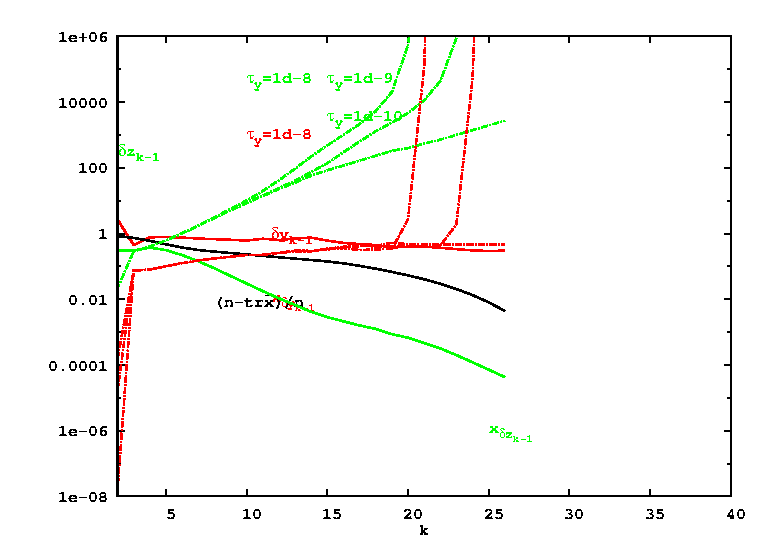
\includegraphics[width=3.5in]{fig_33_tube_cond_10_noscaling/33_nanotube_cond10_noscale_dual.eps}
\caption{Derivatives, displacements and the approximate trace of the unscaled, dual NS iteration for a (3,3) nanotube with $\kappa =10^{10}$.
Derivatives are full lines, whilst the displacements cooresponding to $b=64$, $\tau=10^{-3}$ and $\tau_y=\{10^{-8}, 10^{-9}, 10^{-10}\}$
are the dashed lines.  The trace expectation is shown as a full black line. }
\end{figure}


% \begin{figure}[h]
% 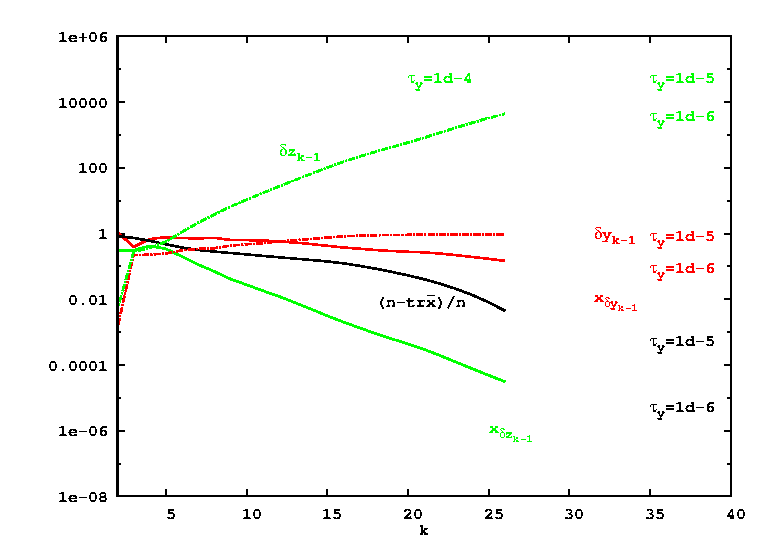
\includegraphics[width=3.5in]{fig_33_tube_cond_10_noscaling/33_nanotube_cond10_noscale_stab.eps}
% \caption{Derivatives, displacements and the approximate trace of the unscaled, stablized NS iteration for a (3,3) 
% nanotube with $\kappa =10^{10}$. 
% Derivatives are full lines, whilst the displacements cooresponding to $b=64$, $\tau=10^{-3}$ and 
% $\tau_y=\{10^{-4}, 10^{-5}, 10^{-6}$  are the dashed lines.  The trace expectation is shown as a full black line. }
% \end{figure}


\begin{figure}[h]
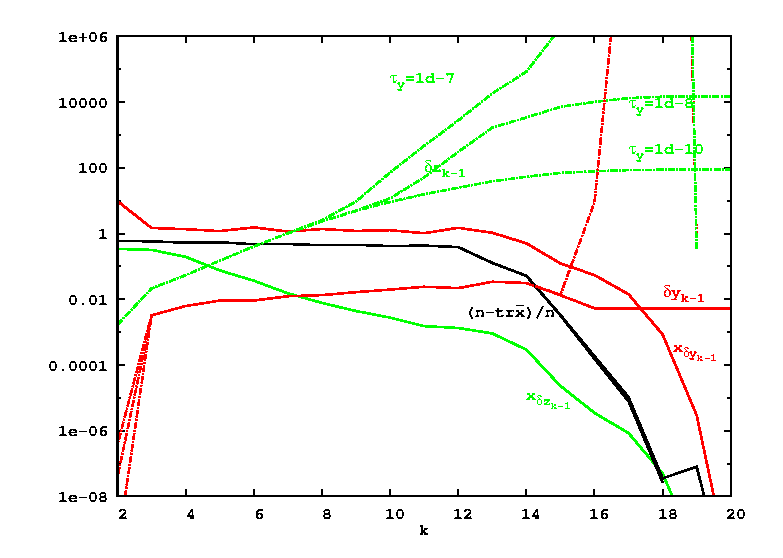
\includegraphics[width=3.5in]{fig_33_tube_cond_10_scaled/33_tube_k10_scale_dual.eps}
\caption{Derivatives, displacements and the approximate trace of the scaled, stablized NS iteration for a
(3,3) nanotube with $\kappa =10^{10}$.
Derivatives are full lines, whilst the displacements cooresponding to $b=64$,
$\tau=10^{-3}$ and $\tau_y=\{10^{-3},10^{-4},10^{-6}\}$
are the dashed lines.  The trace expectation is shown as a full black line. }
\end{figure}

\begin{figure}[h]
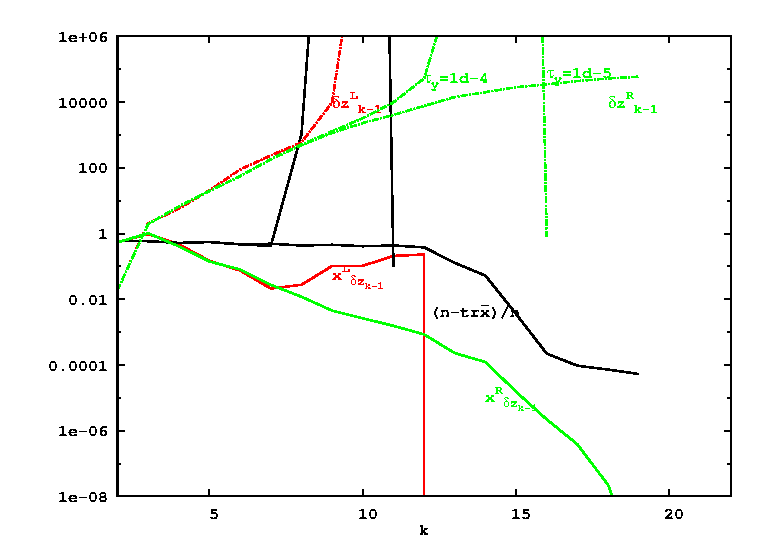
\includegraphics[width=3.5in]{fig_33_tube_cond_10_scaled/33_tube_k10_scale_stab.eps}
\caption{Derivatives, displacements and the approximate trace of the unscaled, dual NS iteration for a (3,3) nanotube with $\kappa =10^{10}$.
Derivatives are full lines, whilst the displacements cooresponding to $b=64$, $\tau=10^{-3}$ and $\tau_y=\{10^{-8}, 10^{-9}, 10^{-10}\}$
are the dashed lines.  The trace expectation is shown as a full black line. }
\end{figure}


<<<<<<< HEAD

\subsection{Lensing}
A feature of square root iteration with the $\ot$ kernel is localization of the culled octree towards identity iteration, 
$\widetilde{\mat{x}}_k \rightarrow \mat{I}\left( \widetilde{\mat{x}}_{k-1} \right)$.  Towards convergence,  
the product $\widetilde{\mat{y}}_k \ot \widetilde{\mat{z}}_k$ involves the product of large and small eigenvalues, and large and small norms, 
which are recursively brought towards unity along the $i=k$ diagonal.  Likewise, application of the NS map, Eq.~(\ref{cannonical}),  tend towards 
reflection about the $ijk$ cube-diagonal.   Because the $\tt SpAMM$ error obeys the multiplicative Cauchy-Schwarz bound, Eq.~(),  the 
cooresponding culled-octree can likewise follow the $i=j$ plane about the $ijk$ cube-diagonal, resolving the {\em relative} error in identity to within $\tau$.    This effect is shown in Figure \ref{x_lensing}.   
We call this identity related,  plane-wise concentration of the culled octree  about the cube-diagonal {\em lensing}.  

Lensing is an algebraic localization offering compression beyond  , 

complexity reduction relative to the naive (full) volume of the cube,
and also relative to sparsification strategies that preserve only absolute errors, as in Eq.~\ref{sparseapprox}.  
The lensed task space offers an enhanced locality of reference, and may also afford fast methods 
with costs approaching an in-place scalar multiply and copy, {\em e.g.} as $h_\alpha \rightarrow \mat{I}$ in Eq.~\ref{cannonical}.
Our thesis is that many problems in physical and information sciences can be brought to this lensed state, {\em e.g.} through preconditioning
as described here, and maintained as the NS residual is brought to a higher level of precision with a more complete $\ot$, 
and also with respect to an outer simulation loop, {\em e.g.} cooresponding to time iteration.



 \begin{figure}[h] \label{markofzorro}
 \fbox{ 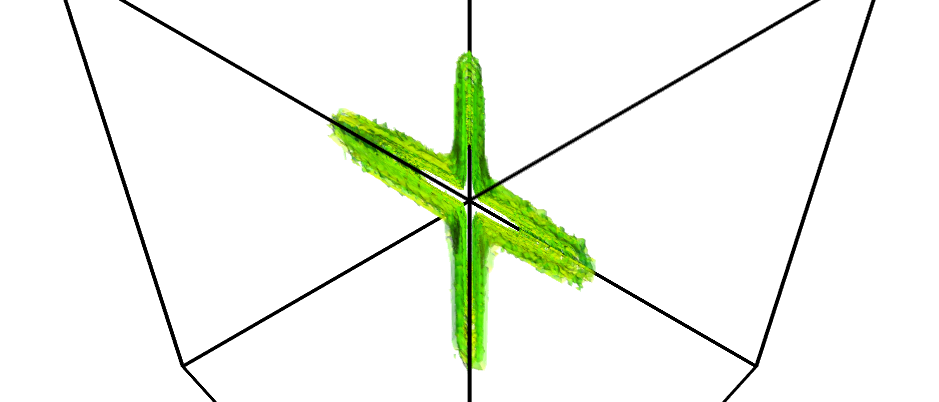
\includegraphics[width=1.in,trim={11.3cm 0cm 11.3cm 0cm},clip]{tube_dual_c6_x128_b64/x_19_scene1.png}} 
 \fbox{ 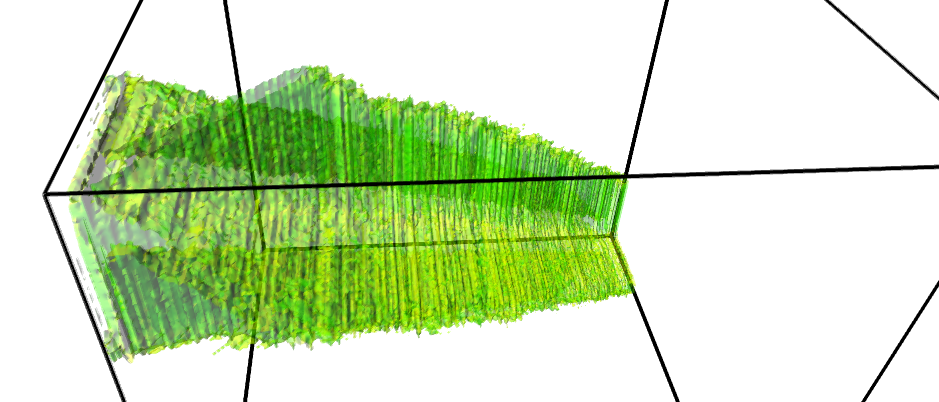
\includegraphics[width=2.in,trim={2cm 0cm 10cm 0cm},clip]{tube_dual_c6_x128_b64/x_19_scene2.png}} 
 \caption{Views of the $\tau =0.03$ sign occlusion surface, for the 
 128x~u.c.~nanotube, at $\sim {14k \times 14k}$ and $\kappa(\mat{s})=10^6$. 
 This surface envelopes the $ijk$ volume of the $\ot$ kernel,  
 cooresponding to the unscaled dual iteration step $\mmat{x}_{19} \leftarrow \mmat{y}_{19} \ot \mmat{z}_{19} $ at $b=64$, $\tau=0.03$ and
 $\tau_y=10^{-3} \, \tau $.  The first pannel looks straight down the cube-diagonal $i=j=k$, from the upper bound towards (1,1,1).
 Remarkably, this surface forms an elongated $\times$, closely following intersection of the $i=j$  and $i=k$ planes 
 along the cube-diagonal. The second pannel looks along the cube-diagonal, with the upper bound at upper left, and (1,1,1) at lower right.}
 \end{figure}

In this section, we present  numerical experiments that highlight the effects of 
ill-conditioning, dimensionality, and the stability of different first order NS approaches to iteration with $\tt SpAMM$. 
We turn first to complexity reduction for $\ot$ in the basin of stability,  where we find a novel, compressive 
effect in the product octree.  This effect is shown in Fig.~\ref{markofzorro},  
for unscaled, inverse square root duals iteration, Eqs.~(\ref{dualsiteration}), on the 3,3 carbon 
nanotube metric at $\kappa=10^6$.  

In this example, the $\tt SpAMM$ octree culled from the $ijk$-cube is outlined by its occlusion surface, enclosing 
a volume that closely follows the $i=j$ and $i=k$ planes, forming an $\times$.  The banded distribution
of large norms along  matrix diagonals leads to cube-diagonal dominance, with plane-following 
a consequence of moderate ill-conditioning,  large norms along the plane-diagonals and their overlap in $ijk$
via the multiplicative bound, Eq.~(\ref{bound}). The tightness of this bound, and the compression gained relative
to  methods that control only the absolute error, {\em e.g.} as given by Eq.~(\ref{sparseapprox}), will hopefully
be quantified in future work. 



\subsection{Metric Locality} 
Metric locality is locality with respect to a Euclidean or generalized distance, {\em e.g.} of the basis.  
=======
\subsection{Metric Locality}
Metric locality is locality with respect to a Euclidean or generalized distance, {\em e.g.} of the basis.
>>>>>>> d4c0ab84d18629f0a3f1847549c555b7d8eece61

\subsubsection{unscaled, with hilbert order}

\subsubsection{unscaled, with salesman's order}

\subsection{Algebraic  Locality}

Reflecting about the cube diagonal is copy in place.  Cooresponds to lensing.


\section{Conversation}

%%eg vs row-col picture.  Example of exact exchange w/DBSR

\bibliography{MatrixFunctions}

\end{document}
